\documentclass[letterpaper]{article}
\usepackage[margin=1in]{geometry}
\usepackage[utf8]{inputenc}
\usepackage{textcomp}
\usepackage{amssymb}
\usepackage{natbib}
\usepackage{graphicx}
\usepackage{gensymb}
\usepackage{amsthm, amsmath, mathtools}
\usepackage[dvipsnames]{xcolor}
\usepackage{enumerate}
\usepackage{mdframed}
\usepackage[most]{tcolorbox}
\usepackage{csquotes}
% https://tex.stackexchange.com/questions/13506/how-to-continue-the-framed-text-box-on-multiple-pages

\tcbuselibrary{theorems}

\newcommand{\R}{\mathbb{R}}
\newcommand{\Z}{\mathbb{Z}}
\newcommand{\N}{\mathbb{N}}
\newcommand{\Q}{\mathbb{Q}}
\newcommand{\C}{\mathbb{C}}
\newcommand{\code}[1]{\texttt{#1}}
\newcommand{\mdiamond}{$\diamondsuit$}
\newcommand{\PowerSet}{\mathcal{P}}
\newcommand{\Mod}[1]{\ (\mathrm{mod}\ #1)}
\DeclareMathOperator{\lcm}{lcm}

%\newtheorem*{theorem}{Theorem}
%\newtheorem*{definition}{Definition}
%\newtheorem*{corollary}{Corollary}
%\newtheorem*{lemma}{Lemma}
\newtheorem*{proposition}{Proposition}


\newtcbtheorem[number within=section]{theorem}{Theorem}
{colback=green!5,colframe=green!35!black,fonttitle=\bfseries}{th}

\newtcbtheorem[number within=section]{definition}{Definition}
{colback=blue!5,colframe=blue!35!black,fonttitle=\bfseries}{def}

\newtcbtheorem[number within=section]{corollary}{Corollary}
{colback=yellow!5,colframe=yellow!35!black,fonttitle=\bfseries}{cor}

\newtcbtheorem[number within=section]{lemma}{Lemma}
{colback=red!5,colframe=red!35!black,fonttitle=\bfseries}{lem}

\newtcbtheorem[number within=section]{example}{Example}
{colback=white!5,colframe=white!35!black,fonttitle=\bfseries}{def}

\newtcbtheorem[number within=section]{note}{Important Note}{
        enhanced,
        sharp corners,
        attach boxed title to top left={
            xshift=-1mm,
            yshift=-5mm,
            yshifttext=-1mm
        },
        top=1.5em,
        colback=white,
        colframe=black,
        fonttitle=\bfseries,
        boxed title style={
            sharp corners,
            size=small,
            colback=red!75!black,
            colframe=red!75!black,
        } 
    }{impnote}
\usepackage[utf8]{inputenc}
\usepackage[english]{babel}
\usepackage{fancyhdr}
\usepackage[hidelinks]{hyperref}
\usepackage{quotes}

\pagestyle{fancy}
\fancyhf{}
\rhead{CSE 100}
\chead{Octber 30th, 2021}
\lhead{``Condensed'' Course Notes}
\rfoot{\thepage}

\setlength{\parindent}{0pt}

\begin{document}

\begin{titlepage}
    \begin{center}
        \vspace*{1cm}
            
        \Huge
        \textbf{CSE 100 Notes}
            
        \vspace{0.5cm}
        \LARGE
        Advanced Data Structures
            
        \vspace{0.5cm}
            
        \large
        A ``Condensed'' Study Guide
        
        \vspace{1.5cm}

        \vfill
            
        Fall 2021\\
        Taught by Professor Niema Moshiri
    \end{center}
\end{titlepage}

\pagenumbering{gobble}

\newpage 

\pagenumbering{gobble}
\begingroup
    \renewcommand\contentsname{Table of Contents}
    \tableofcontents
\endgroup

\newpage
\pagenumbering{arabic}


\section{Introduction to C++}
In this section, we will talk very briefly about C++. We will purposely be omitting:
\begin{itemize}
    \item Templates 
    \item Vectors 
    \item Input/Output 
    \item Some examples.
\end{itemize}

\subsection{Data Types}
\begin{center}
    \begin{tabular}{|c|c|}
        \hline 
        \textbf{Data Type} & \textbf{C++} \\ 
        \hline 
        \code{byte} & 1 byte \\ 
        \code{short} & 2 bytes \\ 
        \code{int} & 4 bytes \\ 
        \code{long} & 8 bytes \\ 
        \code{long long} & 16 bytes \\ 
        \hline 
        \code{float} &  \code{4 bytes} \\ 
        \code{double} & \code{8 bytes} \\ 
        \hline  
        \code{bool} & Usually 1 byte \\ 
        \code{char} & 1 byte \\ 
        \hline 
    \end{tabular}
\end{center}
\textbf{Remark:} In C++, you can have both signed and unsigned data types. 

\subsection{Strings}
Some quick facts about C++ strings in general:
\begin{itemize}
    \item Strings are represented by the \code{string} type.
    \item Strings are actually \underline{mutable}. You can modify strings in-place.
    \item You can only concatenate strings with other strings. So, if you wanted to convert an integer (or any other type) to a string, you would have to \emph{first} convert that integer to a string (or use a string stream). 
    \item We can take the substring using the \code{substr} method. The method signature is:
    \begin{verbatim}
        string#substr(beginIndex, length);
    \end{verbatim}
    \emph{Keep in mind that} C++'s \code{substr} method takes in a \textbf{length} for the second parameter.
\end{itemize}

\subsection{Comparing Non-Primitive Objects}
In C++, even if \code{a} and \code{b} are objects, we can make use of the relational operators:
\begin{verbatim}
    a == b      a != b
    a < b       a <= b
    a > b       a >= b
\end{verbatim}
This is done through something called \textbf{operator overloading}, where we write a custom class and define how these operators should function. A common example of this can be found with \emph{iterators}. 

\subsection{Variables}
Here, we will give a brief overview of variables. 

\subsubsection{Initialization}
Variable initialization in C++ is \textbf{not checked}. Consider the same code, which will compile:
\begin{verbatim}
    int fast;
    int furious; 
    int fastFurious = fast + furious;
\end{verbatim}
Here, this would result in \textbf{undefined} behavior.

\subsubsection{Narrowing}
In C++, we are able to \emph{freely} cast a ``higher'' variable type to a ``lower'' one. No compilation error would occur; that is, the following code would compile:
\begin{verbatim}
    int x = 40_000;
    short y = x;
\end{verbatim}
What would actually happen is that \code{x} would get \textbf{truncated} when it is assigned to \code{y}, resulting in integer overflow. 

\subsubsection{Declaration}
In C++, variables \textbf{can} be declared outside of a class. The following C++ code would compile completely fine: 
\begin{verbatim}
    // MyClass.cpp

    int meaningOfLife = 42;
    class MyClass {
        // some code 
    }
\end{verbatim}
Here, \code{meaningOfLife} is a \textbf{global variable}. Anything in this file can access this variable. In general, it is considered poor practice to use global variables except in cases of constants. 

\subsection{Classes}
Now, we will very briefly go over classes in C++. 

\subsubsection{Class Declaration}
A typical class in C++ looks like: 
\begin{verbatim}
    class Student {
        public: 
            static int numStudents; 

            Student(string n);
            
            void setName(string n);
            string getName() const; 

        private: 
            string name; 
    }

    int Student::numStudents = 0;
    Student::Student(string n) { /* Code */ }
    void Student::setName(string n) { /* Code */ }
    string Student::getName() const { /* Code */ }
\end{verbatim}
A few observations can be made about how classes are laid out. 
\begin{itemize}
    \item In C++, you have a region for your access modifier. That is, there is a \code{public} region, \code{private} region, etc. Any methods or instance variables listed under these regions will take on that access modifier. For instance, \code{setName} is in the \code{public} region, so \code{setName} is public.
    \item In C++, we can ``declare'' the methods and the constructor, and then outside of the class we can implement the methods.
\end{itemize}

\subsubsection{Constructor Shortcut}
Consider the following C++ code:
\begin{verbatim}
    class Point {
        private: 
            int x; 
            int y;
        
        public:
            Point(int i, int j);
    }

    Point::Point(int i, int j) {
        x = i;
        y = j;
    }
\end{verbatim}
This is equivalent to the following: 
\begin{verbatim}
    class Point {
        private: 
            int x; 
            int y;
        
        public:
            Point(int i, int j);
    }

    Point::Point(int i, int j) : x(i), y(j) {}
\end{verbatim}
This is called the \textbf{member initializer list}, and can be used to directly initialize the instance variables. 

\subsection{Memory Management}
Here, we will talk about memory management in C++. 

\subsubsection{Class Copies}
Suppose we have the following C++ code:
\begin{verbatim}
    Student s1("Niema");
    Student s2 = s1;
\end{verbatim}
Here, \code{s1} creates a new \code{Student} instance. \code{s2} \underline{copies} the \code{s1} instance entirely; in other words, it creates a new, \underline{separate} object with the same properties as \code{s1}. The memory diagram for these are shown below: 
\begin{verbatim}
    |-----------------|     |-----------------|
    | |-----------|   |     | |-----------|   |
    | |name: Niema|   |     | |name: Niema|   |
    | |-----------|   |     | |-----------|   |
    |  string object  |     |  string object  |
    |-----------------|     |-----------------|
    Student object          Student object
       s1                       s2
\end{verbatim} 

\subsubsection{References}
Consider the following C++ code: 
\begin{verbatim}
    Student s1 = Student("Niema");
    Student & s2 = s1;
    Student s3 = s2;
\end{verbatim}
The associated memory diagram would look like: 
\begin{verbatim}
    |-----------------|     |-----------------|
    | |-----------|   |     | |-----------|   |
    | |name: Niema|   |     | |name: Niema|   |
    | |-----------|   |     | |-----------|   |
    |  string object  |     |  string object  |
    |-----------------|     |-----------------|
    Student object          Student object 
       s1      s2               s3
\end{verbatim} 
Here, \code{s2} can be seen as \emph{another} way to call \code{s1} (think of \code{s2} as another name for \code{s1}). \code{s3} would be a copy of \code{s1}. 

\subsubsection{Pointers}
Consider the following C++ code: 
\begin{verbatim}
    Student s = Student("Niema");
    // * in this case means pointer 
    // & means memory address
    // So, ptr stores a memory address to some object. In other words, 
    // it points to the object s. 
    Student* ptr = &s; 
    Student** ptrPtr = &ptr; 
\end{verbatim}
The memory diagram would look like: 
\begin{verbatim}
    Mem. Address: 9500 
    |-----------------|
    | |-----------|   |       |-----------|       |-----------|
    | |name: Niema|   |  <--- |    9500   |  <--- |           |
    | |-----------|   |       |-----------|       |-----------|
    |  string object  |       Student* (pointer)   Student** (pointer to pointer) 
    |-----------------|           ptr                  ptrPtr
    Student object      
       s
\end{verbatim} 
If we wanted to access an object through a pointer, we can do this in several ways. 
\begin{enumerate}
    \item Deferencing a pointer. 
    \begin{verbatim}
        // * in this case dereferences the pointer
        // Think of the * as following the arrow  
        (*ptr).name; 
    \end{verbatim}

    \item Arrow dereferencing. 
    \begin{verbatim}
        // ptr->x is the same thing as (*ptr).x
        ptr->name; 
    \end{verbatim}
\end{enumerate}

\subsubsection{Stack/Heap and Dynamic Memory Management}
\begin{verbatim}
    // Same thing as saying 
    // Student s1("Niema");
    Student s1 = Student("Niema");
    Student* s2 = new Student("Ryan");
\end{verbatim}
The corresponding memory diagram is: 
\begin{verbatim}
    |-----------------|     |-----------------|
    | |-----------|   |     | |-----------|   |
    | |name: Niema|   |     | |name: Ryan |   |
    | |-----------|   |     | |-----------|   |
    |  string object  |     |  string object  |
    |-----------------|     |-----------------|
    Student object          Student object 
       s1                                 /|\
                                           |
                                           |
                                           |
                                |------|   |
                                |      | --/
                                |------|
                                Student* (pointer)
                                s2
\end{verbatim}
Here, \code{s1} is allocated on the \emph{stack}; once the method returns, \code{s1} is automatically \underline{destroyed}.

\bigskip 

\code{s2} is allocated through the \code{new} keyword. This is known as dynamic memory allocation. So, \code{s2} is a pointer to the newly allocated memory. Because this object was created using the \code{new} keyword, we need to deallocate it ourselves. To do so, we need to explicitly call \code{delete} on this object: 
\begin{verbatim}
    delete s2; 
\end{verbatim}
\code{delete} takes in a memory address (i.e. pointer). This is very similar to \code{free} (in C). If we don't free this, we run into what is called a \textbf{memory leak}. 

\bigskip 

The variable, \code{s2}, is \textbf{not} allocated on the heap. However, the object that it is pointing to \textbf{is} allocated on the heap. 

\subsection{Constant Keyword}
Now, we will talk about the \code{const} keyword and its significance. 

\subsubsection{The Basics}
In C++, the \code{const} keyword means that the variable can never be reassigned. Consider the following: 
\begin{verbatim}
    const int a = 42; 
    int const b = 42;
\end{verbatim}
If we tried reassigning \code{a} (e.g. \code{a = 41;}), we would get a compiler error. Also, the second line (\code{int const}) is identical to the first line. 

\subsubsection{\code{const} and Pointers}
Consider the following C++ code: 
\begin{verbatim}
    int a = 42;                     // a 
    const int* ptr1 = &a;           // b
    int const* ptr2 = &a;           // c
    int* const ptr3 = &a;           // d
    const int* const ptr4 = &a;     // e
\end{verbatim}
\begin{itemize}
    \item For lines (b) and (c), the pointer cannot modify the object that it is pointing to.  But, we can reassign the pointer to point to a different object. 
    \item For line (d), we cannot reassign the pointer to point to a different object. However, we can modify the object that the pointer is pointing to. 
    \item For (e), we cannot reassign the pointer to point to a different object \emph{or} modify the object that the pointer is pointing to. 
\end{itemize}
In general:
\begin{verbatim}
    const type* const varName = ...; 
    ----------- -------------
       (a)            (b)
\end{verbatim}
\begin{itemize}
    \item Segment (A): The \code{const} next to \code{type*} means that we cannot modify the object or value behind the pointer. 
    \item Segment (B): The \code{const} next to \code{varName} (the variable name) means that we cannot reassign the pointer to point to a different object or value. 
\end{itemize}

\subsubsection{\code{const} and References}
Suppose we have the following C++ code: 
\begin{verbatim}
    int a = 42; 
    const int & ref1 = a;       // a
    int const & ref2 = a;       // b
\end{verbatim}
\begin{itemize}
    \item In (a), the \code{const} means that we cannot modify the variable through the constant reference. So: 
    \begin{verbatim}
        a = 21;         // Allowed. 
        ref1 = 20;      // Compile error!
    \end{verbatim}

    \item (b) is the same exact thing is (a).
\end{itemize}

\subsubsection{\code{const} Functions}
Recall the \code{Student} class from earlier: 
\begin{verbatim}
    class Student {
        public: 
            Student(string n);
            string getName() const; 
            
        private: 
            string name; 
    }

    Student::Student(string n) : name(n) {}
    string Student::getName() const {
        return name;
    }
\end{verbatim}
What does the \code{const} in \code{getName()} do? Well, the \code{const} keyword after the function declaration means that the function cannot modify \emph{this} object. So: 
\begin{itemize}
    \item You cannot do any assignments to instance variables. 
    \item You can only call other \code{const} functions.
\end{itemize} 
So, effectively, \code{const} after a function name means that we are \textbf{guaranteeing} that we aren't changing the object's state in any way.

\subsection{Functions}
In C++, we can have global functions (functions that are defined outside of classes). For instance, the main method (shown below) is a global function (and is required to be):
\begin{verbatim}
    int main() {
        /* Do stuff */ 
    }

    class MyClass {
        /* Some code */ 
    }
\end{verbatim}

\subsubsection{Passing by Value}
In C++, you can pass parameters either by value or reference. 

\bigskip

When passing by value, the function makes a \textbf{copy} of the values that you passed in. Some example code is shown below:
\begin{verbatim}
    void swap(int a, int b) {
        int tmp = a;
        a = b;
        b = tmp;
    }
\end{verbatim}
These copies are destroyed once the function returns (the stack frame is destroyed). 

\subsubsection{Passing by Reference}
When passing by reference, the function takes in \emph{references} to the variables. Some example code is shown below:
\begin{verbatim}
    void swap(int & a, int & b) {
        int tmp = a;
        a = b;
        b = tmp;
    }
\end{verbatim}
Effectively, whatever you change with the references will be reflected with the actual variables. So, in the above \code{swap} method, \code{a} and \code{b} will be updated after the function is done. 

\subsection{Iterators}
Consider the following C++ code: 
\begin{verbatim}
    for (string name : names) {
        cout << name << endl; 
    }
\end{verbatim}
What is \code{names}? 
\begin{itemize}
    \item Is it a \code{vector}? 
    \item Is it a \code{set}? 
    \item Is it an \code{unordered\_set}?
    \item Is it another collection that C++ has? 
\end{itemize}
Well, it doesn't matter! Regardless of what collection we are using, how we use it doesn't matter when it comes to iterating over it. This functionality is made possible by something called \textbf{iterators}.

\subsubsection{Iterating Over Arrays}
Consider the following code: 
\begin{verbatim}
    void printInorder(int* p, int size) {
        for (int i = 0; i < size; ++i) {
            cout << *p << endl; 
            ++p; 
        }
    }
\end{verbatim}
The \code{*p} deferences the pointer, giving the value at the location that the pointer is pointing to. 

\bigskip

The \code{++p} is an example of pointer arithmetic; this will add whatever the size of the type is to the pointer. In this case, this will make the pointer point to the memory address of the next element in the array. 

\bigskip 

Here, we know that \code{p} is (initially) a pointer to the first element in the array: 
\begin{verbatim}
     0   4   8   12  16  20  24  28         Memory Address 
     ------------------------------         (sizeof(int) = 4)
    [10, 20, 25, 30, 46, 50, 55, 60]        Array 
     ^
     p                                      Pointer 
\end{verbatim}
Dereferencing \code{p} (\code{*p}) gives us \code{10}. 

\bigskip 

When we do \code{++p}, we made the pointer point to the next memory address: 
\begin{verbatim}
    0   4   8   12  16  20  24  28         Memory Address 
    ------------------------------
   [10, 20, 25, 30, 46, 50, 55, 60]        Array 
        ^
        p                                  Pointer 
\end{verbatim}
Dereferencing \code{p} (\code{*p}) gives us \code{20}. 


\subsubsection{Using Iterators}
Consider the following C++ code: 
\begin{verbatim}
    vector<string> names; 
    // populate with data 

    vector<string>::iterator itr = names.begin(); 
    vector<string>::iterator end = names.end(); 
    
    while (itr != end) {
        cout << *itr << endl; 
        ++itr; 
    }
\end{verbatim}
Here, we note a few things. 
\begin{itemize}
    \item \code{iterator} is simply a class that handles, well, iteration. So, \code{itr} and \code{end} are instances of the \code{iterator} class that is iterating over \code{names}. 
    \item The \code{!=} operator (in \code{itr != end}) has been overloaded. This checks the \code{curr} property in the \code{iterator} class to see if it is equal (or, more specifically, not equal) to the \code{curr} property of the other index. In this case, \code{itr != end} is effectively comparing \code{itr.curr} with \code{itr.end}. 
    \item The \code{*} dereferencing operator (in \code{*itr}) has also been overloaded. This operator has been overloaded to return whatever the value is at the \code{curr} index. So, in our case,\code{*itr} would return whatever value is at the specified \code{curr} index in the array that we are iterating through. 
    \item The \code{++} operator (in \code{++itr}) is also overloaded. This will increment the \code{curr} property in the \code{iterator} instance. 
\end{itemize}

Suppose \code{names} has the following: 
\begin{verbatim}
        0       1       2           // Index 
    ["Niema", "Ryan", "Felix"]      // names array 
\end{verbatim}

Essentially, \code{vector<string>::iterator} will look something like: 
\begin{verbatim}
    |-----------------------------| |-----------------------------|
    |         |----|              | |         |----|              |
    |   curr: | 0  |              | |   curr: | 3  |              |
    |         |----|              | |         |----|              |
    |           int               | |           int               |
    |-----------------------------| |-----------------------------|
                itr                             end
\end{verbatim}
Calling \code{*itr} will basically give us \code{names[curr]} (or, more specifically, \code{names[0]}). Comparing \code{itr != end} is basically the same as checking \code{0 != 3}. 

\bigskip 

When we call \code{++itr}, we now have: 
\begin{verbatim}
    |-----------------------------| |-----------------------------|
    |         |----|              | |         |----|              |
    |   curr: | 1  |              | |   curr: | 3  |              |
    |         |----|              | |         |----|              |
    |           int               | |           int               |
    |-----------------------------| |-----------------------------|
                itr                             end
\end{verbatim}
Calling \code{*itr} now will basically give us \code{names[curr]} (or, more specifically, \code{names[1]}). Comparing \code{itr != end} is basically the same as checking \code{1 != 3}. 

\subsubsection{Creating an Iterator Class}
When creating data structures, we'll often need to create our own Iterator classes. 

\bigskip 

First, we'll talk about the operators associated with the iterator class: 
\begin{itemize}
    \item \code{==}: \code{true} if the iterators are pointing to the same item and \code{false} otherwise. 
    \item \code{!=}: \code{true} if the iterators are pointing to the different item and \code{false} otherwise. 
    \item \code{*} (dereference): Return a reference to the current data value. 
    \item \code{++} (pre- and post-increment): Move the iterator to the next item. 
\end{itemize}

And, we also need to talk about what functions are in the \underline{data structure class} so we can make use of the iterator:
\begin{itemize}
    \item \code{begin()}: Returns an iterator to the first element. 
    \item \code{end()}: Returns an iterator to the element just after the last element (not the last element, but \emph{after} the last element).  
\end{itemize}
So, in the Linked List example: 
\begin{verbatim}
    [] -> [] -> []
    ^              ^
    begin()        end()
\end{verbatim}
And in any array-based structures: 
\begin{verbatim}
    [a, b, c, d, e]
     ^              ^
     begin()        end()
\end{verbatim}












\newpage
\section{Time and Space Complexity}
One of the key things computer scientists try to do is automate competitive tasks, and of course, that requires \emph{performance}. So, that begs the question: how can we measure the performance of our program? 
\begin{itemize}
    \item How many hours does it take to run? 
    \item Minutes? 
    \item Nanoseconds? 
\end{itemize}
These are all metrics of \emph{human time}. However, a program has two aspects: 
\begin{itemize}
    \item The implementation. 
    \item The algorithm behind that program. 
\end{itemize}
While these different metrics of human time are good at measuring the actual implementation of a program, they don't do a good job describing how fast the \emph{idea}, the algorithm itself, is. For instance, running the algorithm on two different devices, both which have wildly different hardware, will result in a significant difference in how fast your algorithm runs. 

\bigskip 

That being said, we want to know how fast an algorithm is. The best way to do so is by figuring out the performance in terms of number of operations with respect to the input size $n$ (instead of the amount of time). 

\subsection{Notation of Complexity}
Consider the following notations: 
\begin{itemize}
    \item Big-$O$: Upper bound. 
    \item Big-$\Omega$: Lower bound. 
    \item Big-$\theta$: Both upper and lower bound. 
\end{itemize}
Consider the following graph: 
\begin{center}
    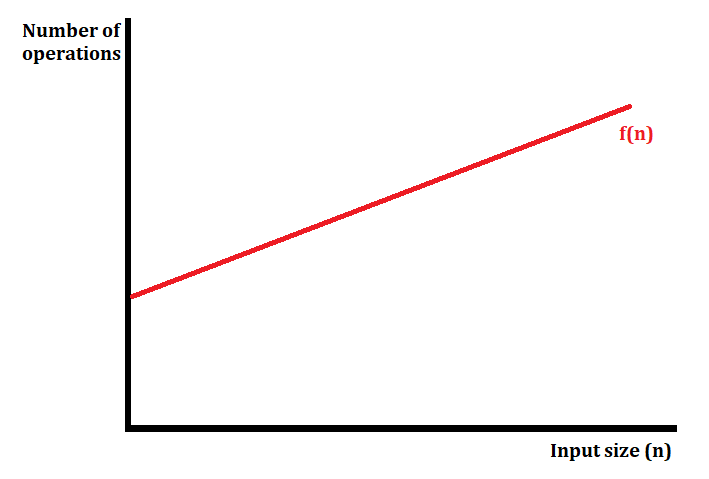
\includegraphics[scale=0.5]{img/graph1.PNG}
\end{center}
Where $f(n)$ describes the number of operations of your algorithm for some $n$. 
\begin{itemize}
    \item We say that $f(n)$ is $O(g(n))$ if, for some constant $a$, we have $a * g(n) \geq f(n)$ as $n \to \infty$. 
    
    \bigskip 

    Consider the following graph: 
    \begin{center}
        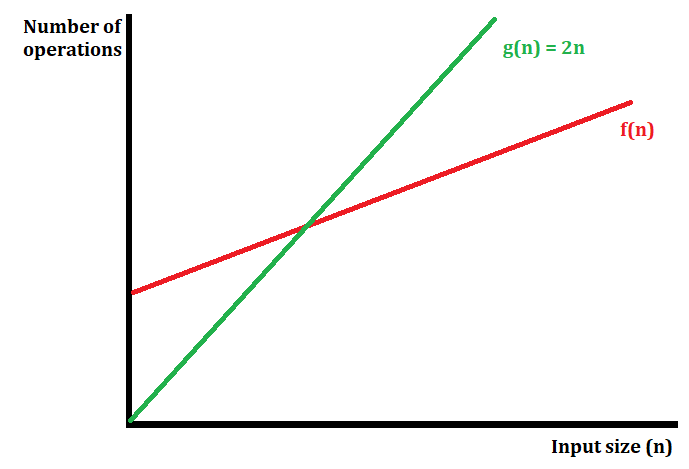
\includegraphics[scale=0.5]{img/graph2.PNG}
    \end{center}
    Here, we see that the intersection of the red and the green line occurs at some point, and that after that point the green line will always be greater than the red line. In other words, at that point, we can say that $f(n)$ will never be bigger than $g(n)$ beyond that point. Therefore, we say that $f(n)$ is $O(2n)$, or simply $O(n)$.
    
    \item Big-$\Omega$ works similarly. We say that $f(n)$ is $\Omega(g(n))$ if, for some constant $b$, $b * g(n) \leq f(n)$ as $n \to \infty$.
    
    \bigskip 

    Consider the following graph: 
    \begin{center}
        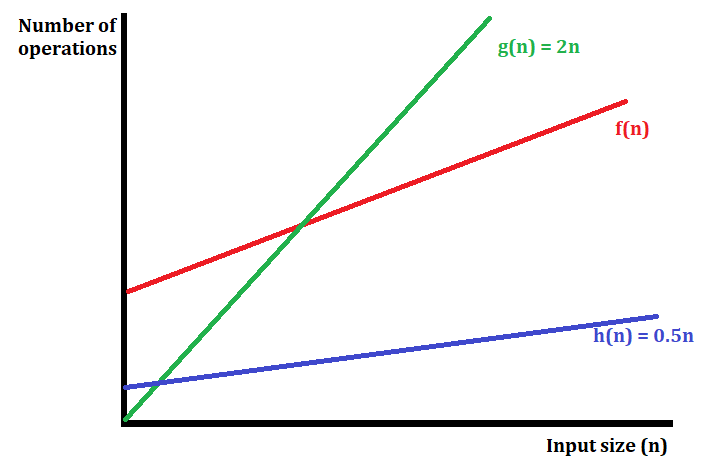
\includegraphics[scale=0.5]{img/graph3.PNG}
    \end{center}
    Here, we see that the blue line $h$ is strictly lower than the red line. In other words, $f(n)$ will never be smaller than $h(n)$. Therefore, we say that $f(n)$ is $\Omega(0.5n)$, or simply $\Omega(n)$. 
    
    \item We say that $f(n)$ is $\theta(g(n))$ if $f(n)$ is $O(g(n))$ and $f(n)$ is $\Omega(g(n))$. Mathematically: 
    \[b * g(n) \leq f(n) \leq a * g(n)\]
    
    In the graphs above, we already found the $b$ and $a$ constants. So:
    \[0.5n \leq f(n) \leq 2n\]
    Therefore, we can say $f(n)$ is $\theta(n)$.
\end{itemize}

\textbf{Remarks:} 
\begin{itemize}
    \item Your bigger or smaller functions do not need to be strictly (i.e. always) bigger or smaller than your $f(n)$. They just need to be strictly bigger or smaller beyond some $n$.
    \item We will almost always use Big-$O$. 
\end{itemize}

\subsection{Common Big-O Time Complexity}
It's good to know of some Big-$O$ time complexities.
\begin{center}
    \begin{tabular}{c|c|p{7cm}}
        Big-$O$ & Common Name & Notes \\ 
        \hline 
        $O(1)$ & Constant & The time complexity does not depend on the input size $n$. \\ 
        $O(\log n)$ & Logarithmic & If the input size is doubled, the number of operations is increased by a constant. One common example is binary search: if we have 8 elements, it would take 3 operations. Doubling the number of elements would result in 4 operations. Also, it does not matter what base the logarithmic function is. \\ 
        $O(n)$ & Linear & Your algorithm scales with the number of elements linearly. For example, twice as many elements roughly means twice as slow. \\ 
        $O(n \log n)$ & & \\ 
        $O(n^2)$ & Quadratic & If the input size is doubled, we'll have quadruple the amount of elements. \\ 
        $O(n^3)$ & Cubic & Similarly to quadratic or linear, if the input size is doubled, the number of operations are multiplied by 8. \\ 
        $O(n^a)$ & Polynomial & For some constant $a$, this is known as polynomial time. All of the Big-$O$ time complexities above are considered polynomial. Anything that is upper-bounded by $O(n^a)$ is called polynomial. \\ 
        $O(k^n)$ & Exponential & For some constant $k$. \\ 
        $O(n!)$ & Factorial &  
    \end{tabular}
\end{center}

\textbf{Remark:} Anything algorithm that runs in polynomial time is considered ``good.'' Exponential and factorial time complexities are considered ``bad.''

\subsection{Space Complexity}
We can also describes algorithms by space complexity -- how much space does an algorithm need for some input size $n$? Just like time complexity, we often use Big-$O$ notation.

\bigskip 

Consider a singly linked list: 
\begin{verbatim}
    |------|     |------|     |------|     |------| 
    | Head | --> |      | --> |      | <-- | Tail | 
    |------|     |------|     |------|     |------|
\end{verbatim}
Suppose it takes $k$ bytes to store a node. If we have $n$ nodes, it would take roughly $k \cdot n$ bytes to represent all of these nodes. We will always have one head and one tail nodes (regardless of how many inputs we have), so these remain constant. Thus, the space complexity for a singly linked list is: 
\[f(n) = kn + 2c\]
Where: 
\begin{itemize}
    \item $c$ is a constant that represents the number of bytes needed to store the head and tail pointer.
    \item $k$ is a constant that represents the number of bytes needed to store a node. 
\end{itemize}













\newpage 
\section{Trees}
Before we can talk about trees, we need to talk about graphs. 

\subsection{Graphs}
A graph is a collection of nodes and edges. For instance, here is a simple graph: 
\begin{verbatim}
           |---|
           | B |
           |---|
          /     \
         /       \
    |---|         |---|
    | A |         | C |
    |---|         |---|
\end{verbatim}
We have nodes $A$, $B$, and $C$, that have some connection to each other. We also have edges, or links, that connect their nodes. 

\bigskip 

There are two types of edges. 
\begin{itemize}
    \item A directed edge, where we can go from one node to another node, but not the other way around. In other words, we can think of a directed edge as an \emph{one-way street}. 
    \item An undirected edge, where we can go from one node to another node and vice versa. In other words, we can think of an undirected edge as a \emph{two-way street}. 
\end{itemize}

With that said, we should observe that the simple graph that we drew above (containing nodes $A$, $B$, and $C$) could represent a linked list. In particular: 
\begin{itemize}
    \item If the edges were undirected, we would have a doubly linked list. 
    \item If the edges were directed (directional), we would have a singly linked list. 
\end{itemize}
So, a linked list is essentially a chain of nodes in sequence. It has $n$ nodes and $n - 1$ edges. 

\subsection{What are Trees?}
A tree is a graph with two properties: 
\begin{itemize}
    \item \underline{It has no undirected cycles.}
    
    \bigskip 

    In graphs, we could theoretically have something like: 
    \begin{verbatim}
               |---|
               | B |
               |---|
              /     \
             /       \
        |---|         |---|
        | A |---------| C |
        |---|         |---|
    \end{verbatim}
    This is known as a \textbf{cycle} (specifically, an undirected cycle). Essentially, we can go from $A$ to $B$, $B$ to $C$, and then back to $A$ from $C$.
    
    \bigskip 

    We can also have something like this: 
    \begin{center}
        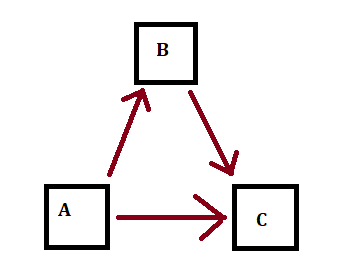
\includegraphics[scale=0.5]{img/graph_dir_cycle.PNG}
    \end{center}
    This is not a cycle because we cannot start at $A$ and end up back at $A$ (and the same applies with $B$). This is because we'll always end up stuck at $C$. And, if we start at $C$, we're stuck at $C$. That being said, if we converted each of the directed edges of this graph into undirected edges, we get an undirected cycle which is not allowed. 

    \item \underline{The nodes must be connected.} 
    
    \bigskip 

    Consider the following graph:
    \begin{verbatim}
        A ---- B

        C ---- D
    \end{verbatim}
    This is not a tree because nodes $A$ and $B$ are not connected to $C$ and $D$. 
\end{itemize}

\subsection{Special Cases of Valid Trees}
There are a few cases of valid trees that we should discuss. 

\begin{itemize}
    \item The empty (``null'') tree. This tree has 0 nodes and 0 edges. 
    \item A tree containing a single node. This has 1 node and 0 edges. 
\end{itemize}

\subsection{Rooted vs. Unrooted Trees}
Now, we talk briefly about rooted vs. unrooted trees. 

\begin{itemize}
    \item A \textbf{rooted} tree is a tree with a hierarchical structure (there is some sense of direction from top to bottom). With a rooted tree, we can consider some definitions:
    \begin{itemize}
        \item For some node, the \textbf{parent} of a node is the node that is directly connected above said node. 
        \item For some node, the \textbf{child} (or \textbf{children}) of a node is/are the node(s) that are directly connected below said node.
        \item The \textbf{root} node is the node at the very top (and thus doesn't have a parent node). 
        \item A node is considered to be a \textbf{leaf} node if it doesn't have any children. 
        \item A node is considered to be an \textbf{internal} node if it does have children. 
    \end{itemize}

    \item An \textbf{unrooted} tree is one where there is not a top-to-bottom hierarchical structure, but more of an inside-outward structure. This looks something like: 
    \begin{verbatim}
        2              6
         \            /
          \          /
           1 ------ 4
          /          \ 
         /            \ 
        3              5
    \end{verbatim}
    With an unrooted tree, we now have the following definitions:
    \begin{itemize}
        \item The \textbf{neighbors} of a node are nodes that are directly connected to said node. For example, node 1 has three neighbor (2, 3, 4). Node 4 also has three neighbor (1, 5, 6).
        \item A node is considered to be a \textbf{leaf} node if it has one neighbor. 
        \item A node is considered to be an \textbf{internal} node if it has more than one neighbor. 
    \end{itemize}
\end{itemize}

\subsection{Rooted Binary Trees}
There are a lot of data structures that involve rooted binary trees. So, let's talk about them. 

\bigskip 

First and foremost, it's rooted (hence the name). This means: 
\begin{itemize}
    \item There is a root node. 
    \item All of the edges have a downward hierarchical relationship. 
\end{itemize}
Trees, in general, do not need to be binary. Any internal node can have any arbitrary number of children. \emph{However}, for a \textbf{binary tree}, any node must have either \underline{0, 1, or 2 child/children nodes}. 

\subsection{Tree Traversals}
If we store our data in some tree data structure, we need a tree traversal algorithm in order to iterate through all nodes (and our data). In this class, we'll talk about the following tree traversal algorithms: 
\begin{itemize}
    \item \textbf{Preorder:} \underline{V}isit, \underline{L}eft, \underline{R}ight. 
    \item \textbf{In-Order:} Left, Visit, Right. 
    \item \textbf{Postorder:} Left, Right, Visit. 
    \item \textbf{Level-Order:} 1st Level (Left to Right), 2nd Level (Left to Right), \dots
\end{itemize} 
We should note that preorder, in-order, and postorder traversals are examples of \textbf{depth first search} (DFS) whereas level-order traversal is an example of \textbf{breadth first search} (BFS). Regardless of the tree traversal algorithm we use, we will always start at the root. 





\newpage 
\section{Binary Search Trees}
A binary search tree is a special type of binary tree with the following properties: 
\begin{itemize}
    \item It must be a rooted binary tree (can only have 0, 1, or 2 children). 
    \item Every node is larger than all nodes in its left subtree. 
    \item Every node is smaller than all nodes in its right subtree. 
\end{itemize}

\subsection{BST Find Algorithm}
Denote \code{query} to be the query (the element we want to find) and \code{current} to be the current node (the node that we're at). The binary search tree find algorithm works as follows
\begin{enumerate}
    \item Start at the root. 
    \item If \code{query == current}, success! 
    \item Otherwise, if \code{query > current}, traverse right and go back to step 2. 
    \item Otherwise, if \code{query < current}, traverse left and go back to step 2. 
\end{enumerate}

\subsection{BST Insert Algorithm}
The binary search tree insert algorithm works as follows
\begin{enumerate}
    \item Perform \code{find} operation, starting at the root. 
    \item If \code{find} succeeds, there is a duplicate element so we don't insert (stop here). 
    \item If \code{find} doesn't succeed, insert the new element at the site of failure. 
\end{enumerate}

\subsection{BST Successor Algorithm}
What is a node successor? Given some node $U$, the successor of node $U$ is the next largest node. In other words, it's the node that is immediately larger than node $U$. If we had an efficient algorithm to determine the successor of a node, then we can implement an efficient iterator that would iterate over our binary search tree in increasing order of size.

\bigskip 

How do we find the successor of a given node? The algorithm is as follows: 
\begin{itemize}
    \item If the node has a right child, traverse right once, then all the way left. 
    \item Otherwise, traverse up the tree. The first time the current node is its parent's left child, the parent is our successor. 
\end{itemize}

\subsection{BST Remove Algorithm}
As usual, we begin by running the find algorithm. However, if we find the node to delete, we need to consider three cases. 

\begin{enumerate}
    \item \underline{No Children:} Just delete the node. 
    \item \underline{One Child:} Just directly connect my child to my parent. 
    \item \underline{Two Children:} Replace my value with my successor's value, and remove me. 
\end{enumerate}

\subsection{Height of a Node and Tree}
\begin{itemize}
    \item The \textbf{height} of a \textbf{node} is the \underline{longest} distance (number of edges) from said node to a leaf. 
    \item The \textbf{height} of a \textbf{tree} is the height of the root of the tree. 
\end{itemize}

\subsection{Tree Balance}
We can think of tree balance as a metric of how tall a tree is with respect to the number of nodes it has. In particular, for some $n$, we can think of tree balancing as a spectrum between perfectly unbalanced and perfectly balanced. 

\bigskip 

Consider $n = 7$ (a tree with 7 nodes).
\begin{verbatim}
    |-------------------------------------------------------------------------------|
    Perfectly Unbalanced                                           Perfectly Balanced 

    1                                                                       4
     \                                                                     / \  
      2                                                                   /   \ 
       \                                                                 /     \ 
        3                                                               /       \ 
         \                                                             2         6 
          4                                                           / \       / \  
           \                                                         /   \     /   \  
            5                                                       1     3   5     7 
             \                                             
              6                                           
               \                                          
                7
\end{verbatim}
In a perfectly unbalanced tree, we have a height of \textbf{6}. In a perfectly balanced tree, we have a height of \textbf{2}. Both trees are binary search trees. 

\bigskip 

Basically, a perfectly unbalanced binary search tree is like a linked list. 

\subsection{Time Complexity}
Part of evaluating the time complexity of any BST is figuring out the tree's shape; whether the tree is balanced or unbalanced will make a difference. 

\bigskip 

For the \code{find}, \code{insert}, and \code{delete} operations, the worst-case runtime is as follows: 
\begin{center}
    \begin{tabular}{c|c|p{7cm}}
        \textbf{Tree Type} & \textbf{Worst Case Big-$O$} & \textbf{Why?} \\
        \hline 
        Perfectly Unbalanced Tree & $\boxed{O(n)}$ & For a perfectly unbalanced tree, if we have $n$ nodes, then a perfectly unbalanced tree will have a height of $n - 1$. The worst case would occur if we had to traverse over all the edges of the tree. \\
        Perfectly Balanced Tree   & $O(\log(n))$ & The reason why this is $O(\log(n))$ -- more specifically, $O(\log_{2}(n + 1) - 1)$ -- is because even if we double the number of nodes in a tree, the tree's height would only grow by 1.
    \end{tabular}
\end{center}
\textbf{Remark:} $O(\log(n))$ is not actually the worst case; this is actually a very nice case simply because this assumes that a tree is perfectly balanced. In other words, \emph{if} the tree was perfectly balanced, the worst-case runtime would be $O(\log(n))$; however, because any given tree will probably not be perfect, we cannot make that assumption. So, the worst-case runtime for any given binary search tree is actually $O(n)$. 

\subsubsection{Find Algorithm: Best vs. Worst vs. Average Case}
We should note that: 
\begin{itemize}
    \item The \textbf{best} case scenario is if the query is the root. 
    \item The \textbf{worst} case scenario is if we need to work with a perfectly unbalanced tree and the query is not found. 
    \item The \textbf{average} case scenario is the theoretical expected value over all trees and queries. 
\end{itemize}

For $n$ elements as $n \to \infty$:
\begin{center}
    \begin{tabular}{c|c|p{7cm}}
        \textbf{Case} & \textbf{Runtime} & \textbf{Remark(s)} \\ 
        \hline 
        Best & $O(1)$ & It doesn't matter if the tree is perfectly balanced or unbalanced if the root node is the right node. \\ 
        Worst & $O(n)$ & If the tree is perfectly unbalanced and the value was either not found or is the last node in the tree (i.e. a leaf node). 
    \end{tabular}
\end{center}

The average case is a bit more complicated. In particular, we need to assume the following:
\begin{enumerate}
    \item All $n$ elements are equally likely to be searched for. 
    
    \bigskip 

    If we had a binary search tree with the elements $1, 2, 3$, then: 
    \[P(Q = 1) = P(Q = 2) = P(Q = 3) = \frac{1}{n} = \frac{1}{3}\]
    This is saying that the probability that our query is \code{1} is the same as the probability that our query is \code{2} which is the same as saying that the probability that our query is \code{3}, or $\frac{1}{3}$. This holds for $n$ elements. 

    \item All $n!$ possible insertion orders are equally likely. 
    
    \bigskip 

    If we had the elements $1, 2, 3$, there are $3! = 6$ possible insertion orders: 
    \begin{itemize}
        \item 123 
        \item 132 
        \item 213
        \item 231
        \item 312
        \item 321 
    \end{itemize}
    \emph{However}, \code{213} and \code{231} gave us the same tree structure. So, there are 5 unique tree structures for 6 possible insertion orders. 
\end{enumerate}

\subsubsection{Depth of a Node}
The \textbf{depth of a node} is the number of nodes in the path from that node to the root. 

\bigskip 

The \textbf{average case time complexity} is the \underline{expected number of operations to find a query}. 

\bigskip 

The average case time complexity is the expected number of operations for every node in this tree. This is equivalent to the \underline{expected depth}. Generally speaking, the number of comparisons to find a node is equal to the depth of that node. 













\newpage 
\section{Treaps and Randomized Search Trees}
Here, we will talk about treaps and randomized search trees, along with a concept called \emph{AVL rotations}.

\subsection{Treap}
A \textbf{treap} is a special tree data structure. The name comes from how this is a \emph{tree} data structure that makes use of a heap. In particular, a treap stores a \code{(key, priority)} pair. 

\bigskip 

How does it make use of both a tree and a heap? 
\begin{itemize}
    \item \textbf{BST} properties with respect to \emph{keys}.
    \begin{itemize}
        \item Larger than all keys in the left subtree. 
        \item Smaller than all keys in the right subtree. 
    \end{itemize}
    In other words, if we ignored the priorities, it would hold the binary search tree properties. 

    \item \textbf{Heap} properties with respect to \emph{priorities}. 
    \begin{itemize}
        \item Larger than all priorities below. 
    \end{itemize}
\end{itemize}

Consider the following valid treap, where the \emph{keys} are the letters and the \emph{priorities} are the numbers: 
\begin{verbatim}
                 (G, 14)
                  /\ 
                 /  \ 
                /    \ 
               /      \ 
            (D, 8)   (L, 10)
             /\         \ 
            /  \         \ 
           /    \         \ 
          /      \         \ 
        (A, 1)  (F, 3)    (T, 5)
\end{verbatim}
With respect to the binary search tree properties: 
\begin{itemize}
    \item We know that $D < G$. 
    \item We know that $A < D$ and $D < F$. 
    \item We know that $G < L$. 
    \item We know that $L < T$. 
\end{itemize}
So, it does fulfill the BST properties. With respect to the keys: 
\begin{itemize}
    \item We know that $14$ is larger than all other nodes (its children); it's also at the top of the tree. 
    \item We know that $8$ is larger than its children nodes ($1 < 3 < 8$). 
    \item We know that $10$ is larger than its child node ($10 > 5$). 
\end{itemize}
So, it does fulfill the Heap properties. 

\subsection{AVL Rotations}
Sometimes, we want to be able to restructure a binary search tree without damaging its binary search tree properties. Here, we make use of something called \textbf{AVL Rotations}.

\bigskip 

Consider the following two trees (here, \code{[a]} means that $a$ is a potential subtree): 
\begin{verbatim}
            b        Right        a
           / \      ------>      / \ 
          /   \                 /   \ 
         a    [z]             [x]    b
        / \          Left            /\
       /   \        <------         /  \
     [x]  [y]                     [y]  [z]
\end{verbatim}
\textbf{Remark:} We can say that, by doing a right AVL rotation, we are rotating $a$ and $b$ clockwise. By doing a left AVL rotation, we are rotating $a$ and $b$ counterclockwise. 

\bigskip 

Regarding the left tree: 
\begin{itemize}
    \item $b$ is the parent node. 
    \item $a$ is a child node with two children. 
    \item $z$ is a right subtree. It could either be one node, an entire subtree, or a \code{nullptr}. 
    \item $x$ is a left subtree (with respect to $a$). It could either be one node, an entire subtree, or empty. 
    \item $y$ is a right subtree (with respect to $a$). It could either be one node, an entire subtree, or empty. 
\end{itemize}
Given the left tree, we can do a \textbf{right AVL rotation}, where: 
\begin{itemize}
    \item We make $a$ the parent. 
    \item We make $b$ become its right child. 
    \item $x$ remains the left child of $a$. 
    \item $z$ remains the right child of $b$. 
    \item We make $y$ the left child of $b$. 
\end{itemize}
More concretely, regarding the left tree: 
\begin{itemize}
    \item We know that $a$ is the left child of $b$. Therefore, $a < b$. 
    \item We know that $z$ is the right child of $b$. That means everything in the $z$ subtree is greater than $b$. Therefore, because $b > a$, it follows that everything in the $z$ subtree is greater than $a$. 
    \item The $x$ subtree is a left descendent of $a$, so all nodes in $x$ is less than $a$ and is therefore less than $b$. 
    \item The $y$ subtree is a right descendent of $a$, so all nodes in $y$ is greater than $a$. 
\end{itemize}
Essentially: 
\begin{verbatim}
    b > a       a < b 
    b < z       a < z
    b > x       a < y
    b > y       a > x
\end{verbatim}
In this particular AVL rotation: 
\begin{itemize}
    \item $x$ (and the edge going into $x$) and $z$ (and the edge going into $z$) remain unchanged. Essentially, this means that $x$ remains a left child of $a$ and $z$ remains a right child of $b$>
    \item Specifically, the only thing that we are changing is are $b$, $a$, and $y$, and their edge relationships. 
\end{itemize}
Why can we make these changes? 
\begin{itemize}
    \item We know that $a < b$ so making $a$ the root node and $b$ a right child node is valid. 
    \item We know that $b > y$ and $a < y$ (or $a < y < b$), so making $y$ the left child of $b$ (where $b$ is the right child of $a$) still maintains the $a < y < b$ property. 
\end{itemize}
When making these changes, the key thing to note is that \underline{we are still maintaining BST properties}. Of course, the same idea applies when doing a \textbf{left AVL rotation}. 

\bigskip 

As a final note, we also consider \emph{kinks}, which require two AVL rotations. In particular, if the nodes are in a kink shape, like so: 
\begin{verbatim}
        a           a       Out-of-balance node. 
       /             \
      b               b     Heavy child node. 
       \             /
        c           c       Heavy grandchild node.
\end{verbatim}
Then, we need to do an AVL rotation on $b$ and $c$ first, and then $a$ and $c$. In other words, we rotate the child and grandchild nodes first, and then the parent and its new child node next. 

\subsection{Treap Insertion}
To insert a new key/priority pair: 
\begin{enumerate}[(1)]
    \item We first insert this pair via the BST insertion algorithm with respect to the keys. 
    \item We use AVL rotations to ``bubble up'' to fix Heap with respect to priorities. 
\end{enumerate}

\subsubsection{Example 1: Simple Treap Insertion}
Recall that the letter represents the key and the number represents the priority. Consider the following treap: 
\begin{verbatim}
            (S, 20)
              / \ 
             /   \
            /     \ 
        (C, 8)  (V, 11)
\end{verbatim}
And let's suppose we wanted to insert $(U, 15)$. 
\begin{enumerate}[(1)]
    \item We first insert this pair like how we would insert any pair by using the BST insertion algorithm. The treap would look something like: 
    \begin{verbatim}
            (S, 20)
              / \ 
             /   \
            /     \ 
        (C, 8)  (V, 11)
                  / 
                 /
             (U, 15)
    \end{verbatim}
    
    \item By inserting this pair, though, we have violated the heap properties. So, we're going to do a \textbf{right AVL rotation} on $U$ and $V$ so that $U$ becomes the new parent. So: 
        \begin{verbatim}
            (S, 20)
              / \ 
             /   \
            /     \ 
        (C, 8)  (U, 15)
                    \  
                     \
                   (V, 11)
    \end{verbatim}
\end{enumerate}


\subsubsection{Example 2: Slightly Harder Treap Insertion}
Recall that the letter represents the key and the number represents the priority. Consider the following treap: 
\begin{verbatim}
                (L, 15)
                  / \ 
                 /   \ 
                /     \ 
               /       \ 
            (E, 8)   (T, 10)
                       / \ 
                      /   \ 
                     /     \ 
                    /       \ 
                  (Q, 5)   (Z, 7)
\end{verbatim}
And let's suppose we wanted to insert $(R, 20)$. 
\begin{enumerate}[(1)]
    \item We first insert this pair like how we would insert any pair by using the BST insertion algorithm. The treap would look something like: 
    \begin{verbatim}
                (L, 15)
                  / \ 
                 /   \ 
                /     \ 
               /       \ 
            (E, 8)   (T, 10)
                       / \ 
                      /   \ 
                     /     \ 
                    /       \ 
                  (Q, 5)   (Z, 7)
                    \ 
                     \ 
                      \ 
                    (R, 20)
    \end{verbatim}
    
    \item By inserting this pair, though, we have violated the heap properties. So, we're going to do a \textbf{left AVL rotation} on $Q$ and $R$ so that $R$ becomes the parent and $Q$ the child.  
    \begin{verbatim}
                (L, 15)
                  / \ 
                 /   \ 
                /     \ 
               /       \ 
            (E, 8)   (T, 10)
                       / \ 
                      /   \ 
                     /     \ 
                    /       \ 
                (R, 20)    (Z, 7)
                  /
                 /
              (Q, 5)
    \end{verbatim}
    The changes we made are: 
    \begin{itemize}
        \item All we did was made $R$ the parent. 
        \item Because $Q < R$, $Q$ is now the left child of $R$. 
    \end{itemize}
    
    \item However, in this position, we are still violating the heap properties. So, we need to do another a \textbf{right AVL rotation} on $R$ and $T$.
    \begin{verbatim}
                (L, 15)
                  / \ 
                 /   \ 
                /     \ 
               /       \ 
            (E, 8)   (R, 20)
                       / \ 
                      /   \ 
                     /     \ 
                 (Q, 5)  (T, 10)
                             \ 
                              \ 
                            (Z, 7)
    \end{verbatim} 
    The changes we made are: 
    \begin{itemize}
        \item $R$ is now the parent. 
        \item $T$ is the right child. 
        \item $R$ keeps the left child. 
    \end{itemize}

    \item Once again, we are still not done since we are still violating the heap properties. So, we need to yet another \textbf{left AVL rotation} on $R$ and $L$ so that $R$ becomes the parent and $L$ the child. 
    \begin{verbatim}
                (R, 20)
                  / \ 
                 /   \ 
                /     \ 
               /       \ 
            (L, 15)   (T, 10)
             / \         \ 
            /   \         \ 
           /     \         \ 
        (E, 8)  (Q, 5)    (Z, 7)
    \end{verbatim} 
    The changes we made are: 
    \begin{itemize}
        \item $R$ is the parent. 
        \item $L$ became the left child. 
        \item $R$'s prior left child ($Q$) became the $L$'s new right child.
        \item Everything else remains unchanged.  
    \end{itemize}

\end{enumerate}


\subsection{Randomized Search Trees (RSTs)}
A randomized search tree is simply a \textbf{treap} where:
\begin{itemize}
    \item We represent the elements as \emph{keys} (thus, maintaining BST properties). 
    \item We \underline{randomly generate} priorities (maintaining heap properties). 
\end{itemize}
In other words, we don't assign a priority level to each element, but a random priority level is assigned to each element for us. 

\bigskip 

Because of the randomness of the priorities, we hope that (on average) we get a better balanced tree. 

\bigskip 

Again, a randomized search tree still has $O(n)$ worst case time complexity because our key/priority pairs could have been formed in a straight linear fashion, and so on. So, we could still get unlucky with the randomly generated numbers. 











\newpage
\section{AVL Trees}
We know that a binary search tree has an average time complexity of $O(\log n)$ and worst time complexity of $O(n)$. Of course, even the average time complexity that we found was derived from some unrealistic assumptions. To mitigate this, we introduced the randomized search tree, which is an extension of a binary search tree that makes the assumptions more reasonable. That being said, the worst case time complexity of a randomized search tree is $O(n)$. What if we wanted the worst time complexity of $O(\log n)$? 

\subsection{Introduction to AVL Trees}
AVL trees are another extension of binary search trees. The only difference, of course, is that it achieves a $O(\log n)$ worst-case for tbe find, insert, and remove operations.

\bigskip 

Before we talk about an AVL tree, we need to talk about some concepts. 
\begin{itemize}
    \item \underline{Balance Factor (BH):} If $R$ is the \underline{height} of the right subtree and $L$ is the \underline{height} of the left subtree, then: 
    \[\text{BH} = R - L\]
    \textbf{Recall:} The \textbf{height} of a \textbf{node} is the \underline{longest} distance (number of edges) from said node to a leaf. 

    \item \underline{AVL Tree:} A binary search tree in which every node has a balance factor of $-1$, $0$, or $1$. 
\end{itemize}

\subsection{Proof of AVL Tree Worst-Case Time Complexity}
We said that worst-case time complexity to find an element in an AVL tree is $O(\log n)$. We need to prove that this is actually the case. 

\begin{mdframed}
    \begin{proof}
        Denote $N_h$ to be the minimum number of nodes that can form an AVL tree with height $h$. Consider, for instance, the following tree: 
    \begin{verbatim}
                [ ]         Root Node 
                / \          
               /   \ 
              /     \ 
             ( )    ( )     Left / Right Subtree 
                              Each subtree can be empty, have one node, 
                              or many nodes. 
    \end{verbatim}
    If this AVL tree has height $h$, we want to minimize the number of nodes that can form this tree. This tree would have, in its entirety, $N_h$ nodes. Suppose we picked an arbitrary subtree, say, the right subtree on the right. Then, this subtree would have a height of $h - 1$ and would thus have $N_{h - 1}$ nodes. By the properties of an AVL tree, we know that the root node can have a balance factor of -1, 0, or 1. The left subtree (in its worst case scenario) would have a height of $h - 2$; this is because the left height plus the root node would give us a height of $h - 2 + 1 = h - 1$, and the right height plus the root node would give us a height of $h - 1 + 1 = h$. So, the balance factor of the root node would be: 
    \[h - (h - 1) = h - h + 1 = 1\]
    Since the left subtree has a height of $h - 2$, it follows that the left subtree has $N_{h - 2}$ nodes. 

    \bigskip 

    We can define a recurrence relation representing the total number of nodes in this tree like so: 
    \[\overbrace{N_h}^{\substack{\text{Total number of} \\ \text{nodes}}} = \underbrace{N_{h - 1}}_{\substack{\text{Number of nodes} \\ \text{in right subtree}}} + \overbrace{N_{h - 2}}^{\substack{\text{Number of nodes} \\ \text{in left subtree}}} + \underbrace{1}_{\text{Root node}}\]
    For this proof only, let's assume that the height of a node is determined by the number of nodes as opposed to the number of edges. For instance, a tree with one node would have a height of 1 and a tree with no nodes would have a height of 0. Then, we know that: 
    \[N_1 = 1\]
    \[N_2 = N_1 + N_0 + 1 = 1 + 1 = 2\]
    Then, we can do: 
    \[N_{h - 1} = N_{h - 2} + N_{h - 3} + 1\]
    \[N_h = (N_{h - 2} + N_{h - 3} + 1) + N_{h - 2} + 1 = 2N_{h - 2} + N_{h - 3} + 2\]
    We know that: 
    \[N_h > 2N_{h - 2}\]
    This is because when we had a tree with $N_h$ nodes, one of the subtrees had $N_{h - 1}$ nodes and the other had $N_{h - 2}$ nodes. By definition, $H_{n - 2}$ is smaller than $H_{n - 1}$. Since, $H_n = N_{h - 2} + N_{h - 1} + 1$, by definition $H_n$ is greater than $2N_{h - 2}$. Therefore: 
    \[N_h > 2^{\frac{h}{2}} \implies \log N_h > \log 2^{\frac{h}{2}} \implies 2\log N_h > h\]
    And, therefore: 
    \[\boxed{h \text{ is } O(\log N_h)}\]
    \end{proof}
\end{mdframed}

\subsection{AVL Tree Insertion}
We now discuss AVL tree insertions. We won't discuss the AVL tree \code{find} algorithm simply because the \code{find} algorithm is equivalent to that of a normal binary search tree's \code{find} algorithm. 

\bigskip 

The insertion algorithm for an AVL tree is slightly more complicated than a normal binary search tree. Specifically, we need to do the following: 
\begin{itemize}
    \item Insert the element like you would with a regular BST insertion. 
    \item After this is done, update balance factors across the tree. 
    \item If any balance factors were broken as a result of this insertion, fix broken balance factors using AVL rotations. 
\end{itemize}






\newpage 
\section{Red-Black Trees}
The red-black tree is a slightly more complicated self-balancing binary search tree. Here, we will talk more about what it is and why we have it. 

\subsection{Properties}
Here are some properties of a red-black tree. 
\begin{enumerate}[(1)]
    \item All nodes must either be \textbf{black} or \textbf{red}. 
    \item The root must be \textbf{black}. 
    \item If a node is \textbf{red}, all of its children must be \textbf{black}. You cannot a \textbf{red} node with a \textbf{red} child. 
    \item For every node $u$, every possible path from $u$ to a \code{null} reference must have the same number of \textbf{black} nodes. A \code{null} reference is \textbf{black}. Essentially, for every single node in the tree, we should be able to take any arbitrary path to get to a \code{null} reference and you should hit the same exact number of black nodes for every single path that could be taken from that given node.
\end{enumerate}

\subsection{Red-Black Trees vs. AVL Trees}
A valid red-black tree is not necessarily a valid AVL tree. 

\subsection{Proof of Red-Black Tree Worst-Case Time Complexity}
We said that the worst-case time complexity to find an element in a red-black tree is $O(\log n)$. We now need to prove that this is the case. 

\begin{mdframed}
    \begin{proof}
        Denote $bh(x)$ to be the number of black nodes from $x$ to a leaf node (excluding itself). Consider the following red-black tree: 
        \begin{verbatim}
                    B
                   / \ 
                  /   \ 
                 B     R
                      / \ 
                     B   B
        \end{verbatim}
        Here, we note that: 
        \begin{itemize}
            \item $bh(\text{root}) = 1$. We exclude the root node when counting the number of nodes, so there is only one other black node. 
            \item $bh(\text{leaf}) = 0$. We cannot count the leaf node itself since we cannot count the initial node. 
            \item $bh(R) = 1$. There are two possible paths from it to a leaf, and on each path there is exactly one black node. 
        \end{itemize}
        Our first claim is: any subtree rooted at $x$ has at least $2^{bh(x)} - 1$ internal nodes. To prove this, we will use induction. 
        \begin{itemize}
            \item \underline{Base Case:} Consider $bh(x) = 0$. This happens when $x$ is a leaf node. So, $2^0 - 1 = 1 - 1 = 0$. This works because the black height of a leaf is 0, and the subtree rooted at a leaf has 0 internal nodes because that subtree only contains that leaf itself.
            \item \underline{Inductive Step:} Let's assume that this claim holds true if the black height is less than $bh(x)$. We now want to show taht this is the case for $bh(x)$. To do so, we need to consider several scenarios (note that $x$ is the root node of the subtree): 
            \begin{itemize}
                \item If $x$ is black and both of its children are black, then it follows that $x$ has $bh(x)$ black height and both child nodes have $bh(x) - 1$ black height. 
                \item If $x$ is black but it has at least one red child, then the red child would have a black height of $bh(x)$ given that $x$ has a black height of $bh(x)$. This is because we do not even count the red node when counting the black height. Whatever number of black nodes we passed from $x$ to a leaf (excluding $x$), we must have passed through the same exact number of nodes through the red child node.
                \item If $x$ is red, then we know that its children must be black (by definition). If $x$ has a black height of $bh(x)$, then both of $x$'s child nodes will have a black height of $bh(x) - 1$ (note that we need to exclude the black node itself when we are calculating its black height). 
            \end{itemize}
            Basically, the number of internal nodes in any possible subtree of $x$ is:
            \[\underbrace{2^{bh(x) - 1} - 1}_{\text{From one child}} + \overbrace{2^{bh(x) - 1} - 1}^{\text{From one child}} + \underbrace{1}_{x \text{ itself}} \geq 2^{bh(x)} - 1\]
            It follows that the claim holds true even in the generalization.  
        \end{itemize}
        Now, denote $h$ to be the height of the tree. In general, at least half of the nodes on any path from the root to the leaf must be black. We are guaranteed that: 
        \[bh(x) \geq \frac{h}{2}\]
        \[n \geq 2^{\frac{h}{2}} - 1\]
        Therefore: 
        \[n + 1 \geq 2^{\frac{h}{2}}\]
        This implies that: 
        \[\log(n + 1) \geq \frac{h}{2}\]
        So, we get that: 
        \[h \leq 2 \log(n + 1)\]
        In other words, $h$ is $O(\log n)$. 
    \end{proof}
\end{mdframed}

\subsection{Red-Black Tree Insertion}
We need to consider a few cases. 

\subsubsection{Insertion Case 1: Empty Tree}
For this, we insert the new node as the root. Then, color that node \textbf{black}. 

\subsubsection{Insertion Case 2: Non-Empty}
We need to do the following: 
\begin{itemize}
    \item Perform regular BST insertion. If you ever see a black node with 2 red children, recolor all three (make the parent red and the children black). In other words: 
    \begin{verbatim}
            B                   R
           / \      ----->     / \ 
          R   R               B   B
    \end{verbatim}
    If the parent is the root, color it black. 

    \item Color the new node \textbf{red}. 
    
    \item Potentially fix the tree for red-black tree properties. This is where we need to consider the potential cases.
    
    \begin{itemize}
        \item \underline{Case 1: Child of Black Node}
        If the new node that we are about to insert is the child of a black node, then we're done.

        \item \underline{Case 2: Child of Red Node, Straight Line}

        Here, we need to: 
        \begin{enumerate}
            \item Insert the node, like normal. 
            \item Perform a single AVL rotation on the upper two nodes. 
            \item Recolor the nodes. 
        \end{enumerate}

        \item \underline{Case 3: Child of Red Node, Kink}
    
        Here, we need to: 
        \begin{enumerate}
            \item Rotate to make straight line. 
            \item Perform straight line insertion case. 
        \end{enumerate}
    \end{itemize}
\end{itemize}








\newpage 
\section{Set and Map ADTs}
Now, we'll talk more about set and map ADTs (abstract data types).

\subsection{The Set ADT}
A set abstract data type is one that stores multiple elements (keys), like an array. It has the following operations: 
\begin{itemize}
    \item \code{find(x)}: \code{true} if \code{x} exists in this set and \code{false} otherwise.
    \item \code{insert(x)}: Add \code{x} to the set. So, whether or not \code{x} was in the set, this operation will make sure \code{x} is in said set. 
    \item \code{remove(x)}: Removes \code{x} from the set.  
\end{itemize}
Notice how we have not discussed any implementation details yet, or what to do if any of these fail (aside from \code{find}). What if we call \code{insert} with an element that already exists in the set? Or, what if \code{remove} is called with an element that doesn't exist in the set? 

\bigskip 

In other words, simply think of a set as a bag of items that has some number of unique elements; you can check if the element exists, insert an element, remove an element, and so on. 

\subsection{The Map ADT}
A map abstract data type is one that stores multiple (key, value) pairs. It has the following operations: 
\begin{itemize}
    \item \code{get(k)}: Returns the value associated with key \code{k} if \code{k} exists in the map.
    \item \code{put(k, v)}: Maps the key \code{k} to the value \code{v}.
    \item \code{remove(k)}: Removes the key \code{k} and its value from the map. 
\end{itemize}
Once again, we have not discussed any implementation details; that is left to whatever ultimately implements this abstract data type. For instance, if we called \code{get} on an key \code{k} that doesn't exist, then should the method return \code{nullptr}? Or throw an error? How about \code{put}? What if the key \code{k} already exists in the map? Should we update the value? Or should we throw an error? 

\bigskip 

For instance, suppose we have a map called \code{students}. Our key could be the student names and the value could be the grades. It would look roughly like: 
\begin{verbatim}
    names (k)       grades (v)
    --------------------------
    Niema      ->   A+ 
    Felix      ->   A 
    Ryan       ->   A
\end{verbatim}
So, with respect to the \emph{keys}, this is essentially a set. In other words, we can think of a map as a set with an associated value. 

\subsection{Implementing the Set and Map ADT}
How can we implement the set and map ADT? We will only briefly discuss how we can implement the set ADT since we can easily transform a set ADT implementation to a map ADT implementation (by storing the key \emph{and} the value as opposed to just the key). The converse is also true; that is, we can transform a map ADT implementation to a set ADT implementation by using dummy values for the values. 

\begin{itemize}
    \item \underline{Unsorted Linked List:} $O(n)$ find/remove, $O(1)$ insert.
    \item \underline{Sorted Linked List:} $O(n)$ find/remove/insert, can iterate in sorted order. 
    \item \underline{Unsorted ArrayList:} $O(n)$ find/remove, amortized $O(1)$ insert. 
    \item \underline{Sorted ArrayList:} $O(\log n)$ find (binary search), $O(n)$ remove/insert, can iterate sorted. 
    \item \underline{Self-Balancing BST:} $O(\log n)$ find/insert/remove, can iterate sorted. 
    \item \underline{Hash Table:} $O(1)$ expected, need to perform $O(k)$ hash where $k$ is a constant representing the length of the key. 
\end{itemize}




\newpage 
\section{Multiway Tries}
In many tree structures, we store elements in the \textbf{nodes} of a tree. Each node represents a single element. A \emph{trie} is a bit different, though. 

\subsection{Trie}
A \textbf{trie} is a tree structure in which elements are represented by \textbf{paths}. Consider the following \emph{binary trie} (a binary trie is a trie that is a binary tree):
\begin{verbatim}
            [ ]
            / \ 
         0 /   \ 1
          /     \ 
        [w]     [ ]
      0 /     0 / \ 1 
       [w]    [w] [w]
\end{verbatim}
Here, we don't even look at the nodes (value-wise). Rather, consider the path from the root node to the left-most leaf node. Here, we note that this path from the root to that leaf node via the edges forms a string of \code{00}. Nodes that are denoted \code{[w]} are word nodes; think of them as separators. In other words, we can choose to \emph{stop} at that node (and get the resulting word) or we can continue until we hit another word node. 

\bigskip

If we take the path to the left-most node and then to the right path followed by the left path, and then the right path fully, we note that this forms the words:  
\begin{verbatim}
    0, 00, 10, 11
     ^   ^   ^ 
    (Word Nodes)

    0 
    0 -> 0 
    1 -> 0
    1 -> 1
\end{verbatim}


\subsection{Multiway Tries}
A \textbf{multiway trie} is a trie in which nodes can have more than \textbf{two children}. 

\bigskip 

Consider the following multiway trie over the DNA alphabet:
\begin{verbatim}
            [ ]
             |
             | T
            [ ]
            / \ 
           /   \ G 
          / A   \ 
         /       \ 
        [ ]      [ ]
      A / \ G    / \ A
      [w] [w]  [w] [w]
\end{verbatim}
Where the DNA alphabet is: 
\[\{A, C, G, T\}\]
The word nodes are denoted by \code{[w]}. We note that the words that can be represented are: 
\begin{itemize}
    \item TAA 
    \item TAG 
    \item TGA 
\end{itemize}

Now, consider the following multiway trie over the English alphabet: 
\begin{verbatim}
            [ ]
             | 
             | A
             |
            [ ]
            / \  T
         D /   \ 
          [w]  [ ]
           |    |
        S  |    | E
          [w]  [w]
\end{verbatim}
The words that are stored are as follows: 
\begin{itemize}
    \item AD 
    \item ADS 
    \item ATE 
\end{itemize}
So, does the word \code{AT} exist in this multiway try? 
\begin{itemize}
    \item The answer is no. While there is a path that consist of \code{AT}, this does not stop at a word node. So, you have \code{ATE}, but not \code{AT}.
\end{itemize}

\subsection{MWT Insertion, Finding, and Removing}
Insertion works like so: 
\begin{itemize}
    \item Start at the root.
    \item For each letter in the word that we are inserting: 
    \begin{itemize}
        \item Check if the current node has a child edge labeled by that letter. 
        \item If it does not, create new child edge labeled by letter.
        \item Traverse down to the node that the end of that child edge. 
    \end{itemize}
    \item Once we finish that word, we mark the current node as a word node. 
\end{itemize}

Finding works like so: 
\begin{itemize}
    \item Start at the root. 
    \item For each letter in the word that we are inserting: 
    \begin{itemize}
        \item Check if the current node has a child edge labeled by that letter. 
        \item If it does not, the word does not exist and we can return. 
        \item Traverse down to the node that the end of that child edge. 
    \end{itemize}
    \item Check if the node is a word node. If it is, the word is found. Otherwise, it is not found. 
\end{itemize}

Deleting works like so: 
\begin{itemize}
    \item Start at the root. 
    \item For each letter in the word that we are inserting: 
    \begin{itemize}
        \item Check if the current node has a child edge labeled by that letter. 
        \item If it does not, the word does not exist and we can return. 
        \item Traverse down to the node that the end of that child edge. 
    \end{itemize}
    \item Check if the node is a word node. If it is, unmark it as a word node (so that it doesn't form a word). 
\end{itemize}










\newpage 
\section{Ternary Search Trees}
A ternary search tree serves a similar purpose to a multiway trie. However, performance-wise, there are differences. 
\begin{itemize}
    \item \underline{BST:} $O(k \log n)$, memory efficient. 
    \item \underline{MWT:} $O(k)$, memory inefficient. 
    \item \underline{TST:} Somewhere in between. It stores words similarly to a MWT, but with less wasted speed. 
\end{itemize}
One notable difference between MWTs and TSTs is how we use \textbf{nodes} to store a letter.

\subsection{TST Find Algorithm}
The find algorithm for a ternary search tree works like so: 
\begin{itemize}
    \item Start at the root node. Denote $N$ as the node that we are at and $N_l$ as the letter at this node. 
    \item For each letter $l$ in the query: 
    \begin{itemize}
        \item If $l > N_l$, then traverse to the right child node. 
        \item Else, if $l < N_l$, then traverse to the left child node. 
        \item Else, we do the following: 
        \begin{itemize}
            \item If $l$ is the last letter of the query and $N$ is a word node, then we found the word. 
            \item Else, traverse to the middle child. 
        \end{itemize}
    \end{itemize}
    \item At this point, the word wasn't found, so it doesn't exist. 
\end{itemize}

\subsection{TST Insert Algorithm}
The idea behind this algorithm is very similar in nature to the TST find algorithm. The notable differences are: 
\begin{itemize}
    \item If we need to traverse to a child that doesn't exist, simply create it and traverse. 
    \item Make the last word in the traversal a word node. 
\end{itemize}

\subsection{TST Remove Algorithm}
Again, the idea behind this algorithm is very similar in nature to the TST find algorithm. The only difference is: 
\begin{itemize}
    \item Make the last node in the traversal not a word node. 
\end{itemize}

\subsection{TST Time Complexity}
The time complexity for a TST is: 
\begin{itemize}
    \item $O(n)$ worst case. 
    \item $O(\log n)$ average case. 
\end{itemize}








\newpage 
\section{Appendix}
Here's some useful information that might be helpful. 

\subsection{Lecture and Stepik Links}
These all link to the corresponding lectures on Edstem and Stepik. You may need to be logged in.
\begin{center}
    \begin{tabular}{|c|c|c|c|}
        \hline 
        \textbf{Num.} & \textbf{Lecture Title} & \textbf{Edstem Link} & \textbf{Stepik Link} \\ 
        \hline 
        1 & Course Introduction & \href{https://edstem.org/us/courses/6609/lessons/22848/slides/131953}{Click Here} & N/A \\ 
        2 & C++ Review & \href{https://edstem.org/us/courses/6609/lessons/22849/slides/131958}{Click Here} & \href{https://stepik.org/lesson/26055/step/1?unit=8087}{Click Here} \\ 
        3 & C++ Iterators & \href{https://edstem.org/us/courses/6609/lessons/22850/slides/131970}{Click Here} & \href{https://stepik.org/lesson/26105/step/1?unit=11291}{Click Here} \\ 
        4 & Time and Space Complexity & \href{https://edstem.org/us/courses/6609/lessons/22853/slides/131982}{Click Here} & \href{https://stepik.org/lesson/26053/step/1?unit=8085}{Click Here} \\ 
        5 & Trees & \href{https://edstem.org/us/courses/6609/lessons/22854/slides/131990}{Click Here} & \href{https://stepik.org/lesson/28726/step/1?unit=9784}{Click Here} \\ 
        6 & Binary Search Trees & \href{https://edstem.org/us/courses/6609/lessons/22855/slides/131996}{Click Here} & \href{https://stepik.org/lesson/28727/step/1?unit=9785}{BSTs}/\href{https://stepik.org/lesson/28730/step/1?unit=9787}{BST Avg. Time-Complex} \\ 
        7 & Treaps and Randomized Search Trees & \href{https://edstem.org/us/courses/6609/lessons/22858/slides/132012}{Click Here} & \href{https://stepik.org/lesson/28863/step/1?unit=9900}{Heaps}/\href{https://stepik.org/lesson/28864/step/1?unit=9901}{RSTs} \\ 
        8 & AVL Trees & \href{https://edstem.org/us/courses/6609/lessons/22859/slides/132019}{Click Here} & \href{https://stepik.org/lesson/28865/step/1?unit=9903}{Click Here} \\ 
        9 & Red-Black Trees & \href{https://edstem.org/us/courses/6609/lessons/22860/slides/132026}{Click Here} & \href{https://stepik.org/lesson/28866/step/1?unit=9902}{Click Here} \\ 
        10 & Set and Map ADTs & \href{https://edstem.org/us/courses/6609/lessons/22863/slides/132039}{Click Here} & \href{https://stepik.org/lesson/30821/step/1?unit=11598}{Lexicon}/\href{https://stepik.org/lesson/31305/step/1?unit=11644}{LL}/\href{https://stepik.org/lesson/31306/step/1?unit=11645}{Array}/\href{https://stepik.org/lesson/31307/step/1?unit=11646}{BSTs}/\href{https://stepik.org/lesson/31308/step/1?unit=11647}{HT/HM} \\ 
        11 & Multiway Trie & \href{https://edstem.org/us/courses/6609/lessons/22864/slides/132045}{Click Here} & \href{https://stepik.org/lesson/30819/step/1?unit=11596}{Click Here} \\ 
        12 & Ternary Search Tree & \href{https://edstem.org/us/courses/6609/lessons/22865/slides/132054}{Click Here} & \href{https://stepik.org/lesson/30820/step/1?unit=11597}{Click Here} \\ 
        \hline 
    \end{tabular}
\end{center}


\subsection{Visualization Links}
Click \href{here}{https://www.cs.usfca.edu/~galles/visualization/Algorithms.html} to see all visualizations. Some important ones: 
\begin{center}
    \begin{tabular}{|c|c|}
        \hline 
        \textbf{Data Structure} & \textbf{Link} \\ 
        \hline 
        Binary Search Tree & \href{https://www.cs.usfca.edu/~galles/visualization/BST.html}{Click Here} \\ 
        AVL Trees & \href{https://www.cs.usfca.edu/~galles/visualization/AVLtree.html}{Click Here} \\ 
        Red-Black Trees & \href{https://www.cs.usfca.edu/~galles/visualization/RedBlack.html}{Click Here} \\ 
        Trie & \href{https://www.cs.usfca.edu/~galles/visualization/Trie.html}{Click Here} \\ 
        Ternary Search Tree & \href{https://www.cs.usfca.edu/~galles/visualization/TST.html}{Click Here} \\ 
        \hline 
    \end{tabular}
\end{center}

\subsection{Time/Space Complexities}
Here are some time/space complexities, courtesy of Wikipedia. 

\subsubsection{Binary Search Tree}
\begin{center}
    \begin{tabular}{|c|c|c|}
        \hline 
        \textbf{Algorithm} & \textbf{Average} & \textbf{Worst} \\ 
        \hline 
        Search/Find & $O(\log n)$ & $O(n)$ \\ 
        Insert & $O(\log n)$ & $O(n)$ \\ 
        Delete & $O(\log n)$ & $O(n)$ \\ 
        \hline 
    \end{tabular}
\end{center}

Space Complexity: 
\begin{itemize}
    \item Average: $O(n)$ 
    \item Worst: $O(n)$
\end{itemize}


\subsubsection{Treap/RST}
\begin{center}
    \begin{tabular}{|c|c|c|}
        \hline 
        \textbf{Algorithm} & \textbf{Average} & \textbf{Worst} \\ 
        \hline 
        Search/Find & $O(\log n)$ & $O(n)$ \\ 
        Insert & $O(\log n)$ & $O(n)$ \\ 
        Delete & $O(\log n)$ & $O(n)$ \\ 
        \hline 
    \end{tabular}
\end{center}

Space Complexity: 
\begin{itemize}
    \item Average: $O(n)$ 
    \item Worst: $O(n)$
\end{itemize}


\subsubsection{AVL Tree}
\begin{center}
    \begin{tabular}{|c|c|c|}
        \hline 
        \textbf{Algorithm} & \textbf{Average} & \textbf{Worst} \\ 
        \hline 
        Search/Find & $O(\log n)$ & $O(\log n)$ \\ 
        Insert & $O(\log n)$ & $O(\log n)$ \\ 
        Delete & $O(\log n)$ & $O(\log n)$ \\ 
        \hline 
    \end{tabular}
\end{center}

Space Complexity: 
\begin{itemize}
    \item Average: $O(n)$ 
    \item Worst: $O(n)$
\end{itemize}


\subsubsection{Red-Black Tree}
\begin{center}
    \begin{tabular}{|c|c|c|}
        \hline 
        \textbf{Algorithm} & \textbf{Average} & \textbf{Worst} \\ 
        \hline 
        Search/Find & $O(\log n)$ & $O(\log n)$ \\ 
        Insert & Amortized $O(1)$ & $O(\log n)$ \\ 
        Delete & Amortized $O(1)$ & $O(\log n)$ \\ 
        \hline 
    \end{tabular}
\end{center}
\textbf{Remark:} The below quote is from Stepik. 
\begin{quote}
    The balance restrictions of the AVL Tree are stricter than those of the Red-Black Tree, so even though the two data structures have the same time complexities, in practice, AVL Trees are typically faster with find operations (because they are forced to be more balanced, so traversing down the tree without modifying it is faster) and Red-Black Trees are typically faster with insertion and removal operations (because they are not required to be as balanced, so they perform less operations to maintain balance after modification).
\end{quote}

Space Complexity: 
\begin{itemize}
    \item Average: $O(n)$ 
    \item Worst: $O(n)$
\end{itemize}


\subsubsection{Multiway Trie}
\begin{center}
    \begin{tabular}{|c|c|c|}
        \hline 
        \textbf{Algorithm} & \textbf{Worst} \\ 
        \hline 
        Search/Find & $O(k)$ \\ 
        Insert & $O(k)$ \\ 
        Delete & $O(k)$ \\ 
        \hline 
    \end{tabular}
\end{center}
Here, $k$ is the length of the word. 

\bigskip 

Space Complexity: 
\begin{itemize}
    \item Worst: $O(\Sigma^k)$, where $\Sigma$ is the size of the alphabet and $k$ is the size of a word. 
\end{itemize}


\subsubsection{Ternary Search Tree}
\begin{center}
    \begin{tabular}{|c|c|c|}
        \hline 
        \textbf{Algorithm} & \textbf{Average} & \textbf{Worst} \\ 
        \hline 
        Search/Find & $O(\log n)$ & $O(\log n)$ \\ 
        Insert & $O(\log n)$ & $O(\log n)$ \\ 
        Delete & $O(\log n)$ & $O(\log n)$ \\ 
        \hline 
    \end{tabular}
\end{center}

Space Complexity: 
\begin{itemize}
    \item Average: $O(n)$ 
    \item Worst: $O(n)$
\end{itemize}

\end{document}